%═══════════════════════════════════════════════════════════════════════════════
\section{Designing Evidence for a Decision}\label{sec:choosing}
%═══════════════════════════════════════════════════════════════════════════════

The previous section left a problem. Many profiles are valid, and they
can lead the decision-maker to different actions, so validity alone cannot
tell the statistician which profile to report. Something else has to decide.

The decision-maker first has to name the action they want the profile to
support, called the target. Which action they name reflects their attitude
toward risk. A decision-maker who wants the
strongest guarantee names the action with the smallest worst-case expected
loss across the model, called the protective action. One who trusts the
belief names the action with the smallest expected loss under the belief,
i.e. the action that would cost least on average if the belief were true.

With the target named, the statistician designs the profile, and three
results show how. The first finds the profile that gives the target the
strongest guarantee. The second shows how to trade some of that guarantee for
information without losing the target. The third shows that the standard
construction, which reshapes the likelihood ratio, cannot in general find the
first.

\subsection{Result 1: the Safest Profile for an Action}\label{sec:result1}

Start with protection. Fix an action $d$. Its certificate $C(d;\mathcal E)$
bounds the expected loss of $d$ under every distribution in the model, so the
lower the certificate, the stronger the guarantee. The question is how low a
valid profile can push it.

The answer can be guessed. The certificate is the largest of the ratios
$L(d,z)/\mathcal E(z)$, one for each outcome. To keep the largest one small,
the profile should put large scores where the action is expensive. But the
scores share a budget, so a large score on one outcome means a smaller score
elsewhere. The best compromise is to make all the ratios equal, so that none
is larger than it needs to be, and that means scores proportional to the
losses. The theorem confirms this.

\begin{theorem}[Certificate optimum]\label{thm:cert}
Fix an action $d\in\mathcal D$ and let
\[
  \mu_d:=\max_{P\in\mathcal P}\mathbb E_{P}[L(d,Z)]
\]
be its worst expected loss across the model, assumed strictly positive and
attained by some $P^\star\in\mathcal P$. Every valid e-variable
$\mathcal E$ satisfies
\[
  C(d;\mathcal E)\geq\mu_d,
\]
where $C(d;\mathcal E)$ is the certificate \eqref{eq:wl_decision},
and equality is attained by
\[
 \mathcal E_d^{\mathrm{safe}}(z)=\frac{L(d,z)}{\mu_d}.
\]
Moreover this profile is the only one attaining the bound: any valid
$\mathcal E$ with $C(d;\mathcal E)=\mu_d$ equals $\mathcal E_d^{\mathrm{safe}}$
at every outcome.
\end{theorem}

\begin{proof}
Let $\mathcal E$ be a valid e-variable and write $C:=C(d;\mathcal E)$ for
its certificate. If $C=\infty$ the bound is immediate, so assume $C<\infty$.
Since $C$ is the largest of the ratios $L(d,z)/\mathcal E(z)$, every outcome
satisfies $L(d,z)\leq C\,\mathcal E(z)$. Taking expectations of both sides
under $P^\star$ gives
\[
  \mu_d=\mathbb E_{P^\star}[L(d,Z)]
  \leq C\,\mathbb E_{P^\star}[\mathcal E(Z)]
  \leq C,
\]
where the final inequality is validity of $\mathcal E$ under $P^\star$. This
proves the lower bound.

For attainment, $\mathcal E_d^{\mathrm{safe}}$ is non-negative and valid,
because for every $P\in\mathcal P$
\[
  \mathbb E_{P}[\mathcal E_d^{\mathrm{safe}}]
  =\frac{\mathbb E_{P}[L(d,Z)]}{\mu_d}\leq1,
\]
the inequality holding because $\mu_d$ is the largest such expected loss,
with equality at $P=P^\star$. The safe profile is therefore exact under
$P^\star$, spending its whole budget there. Where
$L(d,z)>0$ the ratio $L(d,z)/\mathcal E_d^{\mathrm{safe}}(z)$ equals $\mu_d$,
and where $L(d,z)=0$ it equals zero under the convention $0/0=0$. Since
$\mu_d>0$, at least one outcome has $L(d,z)>0$, so the largest ratio is
$\mu_d$.

For uniqueness, suppose a valid $\mathcal E$ attains $C=\mu_d$. Both
inequalities in the displayed chain are then equalities. The second forces
$\mathbb E_{P^\star}[\mathcal E]=1$, so every optimal profile is exact under
$P^\star$, and the first forces
\[
  \sum_{z\in\mathcal Z}P^\star(z)\bigl(\mu_d\,\mathcal E(z)-L(d,z)\bigr)=0 .
\]
Every bracket is non-negative and every $P^\star(z)$ is strictly positive, so a
sum of non-negative terms can vanish only if each term does. Hence
$\mu_d\,\mathcal E(z)=L(d,z)$ at every outcome, which is
$\mathcal E=L(d,\cdot)/\mu_d$.
\end{proof}

In words, the best guarantee any valid profile can give $d$ is its
worst-case expected loss $\mu_d$, and only one profile achieves it, the one
that scores each outcome in proportion to what $d$ costs there. Call it the
safe profile for $d$.

Three features of the safe profile matter below. First, only one member of
the model is relevant. Validity holds with equality under $P^\star$, the
distribution under which $d$ looks worst, and with room to spare under members
that make $d$ look cheaper, so adding members to the model changes nothing
unless one of them makes $d$ look worse than $P^\star$ does.

Second, the best
guarantee available for any action is
\[
  \min_{d\in\mathcal D}\ \max_{P\in\mathcal P}\mathbb E_{P}[L(d,Z)],
\]
which the protective action attains. Third, the safe profile never uses the
belief. It is built from the loss and the model alone, so a decision-maker who
wants only the strongest guarantee has no use for the belief. That is not a
defect of the belief, but what wanting only protection means.

A guarantee for an action is only useful if the decision-maker, handed the
profile, actually takes that action. The rule compares all actions under the
same profile, so a competitor could in principle come out cheaper. The next
result shows that this happens only if the target was a poor choice to begin
with.

\begin{corollary}[The safe profile selects its action]\label{cor:select}
Under the conditions of Theorem~\ref{thm:cert}, $\mathcal E_d^{\mathrm{safe}}$
weakly selects $d$, meaning $d$ is among the actions the rule returns,
unless some competitor $d'$ costs less than $d$ in every outcome where $d$ costs anything and nothing where $d$ costs nothing. In
particular, it weakly selects any action that is cheapest against the model,
and any action that is cheapest under a distribution giving every outcome
positive probability.
\end{corollary}

\begin{proof}
Under $\mathcal E_d^{\mathrm{safe}}$ the target's certificate is $\mu_d$, and
a competitor's is
\[
  C(d';\mathcal E_d^{\mathrm{safe}})
  =\mu_d\max_{z\in\mathcal Z}\frac{L(d',z)}{L(d,z)},
\]
with the conventions of \eqref{eq:wl_decision}. This falls below $\mu_d$
exactly when every ratio is below one, which is the stated condition. An
action cheapest against the model cannot be beaten, since by
Theorem~\ref{thm:cert} every competitor has
$C(d';\mathcal E)\geq\mu_{d'}\geq\mu_d$. An action cheapest under a
distribution $Q$ with full support cannot be beaten either, since a competitor
meeting the condition would have strictly smaller expected loss under $Q$.
\end{proof}

In other words, the safe profile can hand the decision only to an action
that is cheaper than the target in every outcome, and no decision-maker would
target an action like that. It may tie with a competitor, which is why
selection is only weak.

\subsection{Result 2: Informing Is Not Inducing}\label{sec:result2}

The safe profile gives the target the strongest guarantee, but it ignores
the belief entirely. A decision-maker who also wants the evidence to reflect
the belief needs something else. The standard answer is the likelihood ratio
$r$ of \eqref{eq:intro_lr}, the valid profile that maximises expected
log-evidence under the belief \citep{Grunwald2024safe,Koning2025continuous}.
The natural question is whether it leads to the target. It need not, even
when the target is the action the belief itself recommends.

Take the two-outcome example, where the belief favours the bet $d_1$. There
$P_0=(1/2,1/2)$ and $\widehat P_1=(0.75,0.25)$, so $r=(1.5,0.5)$, and with
$L(d_1,\cdot)=(0,8)$ and $L(d_2,\cdot)=(4,0)$ the certificates are
\[
  C(d_1;r)=\max\bigl(0/1.5,\;8/0.5\bigr)=16,
  \qquad
  C(d_2;r)=\max\bigl(4/1.5,\;0/0.5\bigr)=8/3 .
\]
The rule selects the hedge $d_2$. The reason is where the ratio puts its
scores. It puts the large score on $A$, the outcome the belief expects, and
the small score on $B$, the only outcome in which the bet loses anything.
Dividing the bet's loss of $8$ by $0.5$ doubles it instead of shrinking it.
The profile that best reflects the belief leads the decision-maker away from
the action the belief recommends.

So information and the target can conflict, and the target has to come first.
The decision-maker names the target, written $d^\star$, and the statistician
looks for the most informative profile among those that lead to it. A natural
target is the action the belief recommends,
\[
 d^\star\in\argmin_{d\in\mathcal D}
 \mathbb E_{\widehat P_1}[L(d,Z)],
\]
though any target the decision-maker names is handled the same way. The
target is fixed before the profile is designed, so it does not depend on
$\mathcal E$. What depends on $\mathcal E$ is the action the rule returns,
$\delta(\mathcal E)$, and the requirement is that this action be $d^\star$.

Information is measured, as in Section~\ref{sec:intro_two}, by expected
log-evidence under the belief, $\mathbb E_{\widehat P_1}[\log\mathcal E(Z)]$.
The problem is then
\begin{equation}
 \begin{aligned}
 \max_{\mathcal E}\quad &\mathbb E_{\widehat P_1}[\log\mathcal E(Z)]\\
 \text{subject to}\quad
 &\mathcal E\geq0,\qquad
 \mathbb E_{P}[\mathcal E(Z)]\leq1\ \ \text{for all }P\in\mathcal P,\\
 &d^\star\in\argmin_{d\in\mathcal D}C(d;\mathcal E).
 \end{aligned}
 \label{eq:constrained_log}
\end{equation}
The first line of constraints says the profile is valid, and without the
second line the answer would be the likelihood ratio. The second line is a
constraint on the profile. It keeps only profiles under which the rule
returns $d^\star$, however informative the others are, so it changes the
answer only when the likelihood ratio leads elsewhere, as in the example.

What does the answer look like then? The next result shows that it sits
exactly where the target stops winning.

\begin{proposition}[Boundary structure]\label{prop:boundary}
Assume in addition that $\mathcal D$ is finite, that $\widehat P_1(z)>0$ for
every outcome, so that expected log-evidence is finite inside the feasible set
and strictly increasing in every coordinate, and that exactly one validity
constraint binds at the optimum. Write $P^\star$ for the member it binds
under, which is $P_0$ for a one-point model, and $r=\widehat P_1/P^\star$.
Let
\[
 F=\{\mathcal E\geq0:\ \mathbb E_{P}[\mathcal E]\leq1\ \text{for all }P\in\mathcal P,\;
 d^\star\in\argmin_d C(d;\mathcal E)\}
\]
be the feasible set of \eqref{eq:constrained_log}, and let $\mathcal E^\star$
be a maximiser of expected log-evidence over $F$ with a finite objective. Then
validity binds at $\mathcal E^\star$. If $d^\star$ is strictly selected at
$\mathcal E^\star$, meaning its certificate is strictly smaller than every
competitor's, then $\mathcal E^\star=r$. Consequently, if $r$ does not select
$d^\star$, the target ties with some competitor $d'$ at the optimum,
$C(d^\star;\mathcal E^\star)=C(d';\mathcal E^\star)$, and is only weakly
selected.
\end{proposition}

\begin{proof}
If every validity constraint is slack at $\mathcal E^\star$, scaling
$\mathcal E^\star$ by a constant $c>1$ raises the objective, which is strictly
increasing in each coordinate, and scales every certificate by $1/c$,
preserving the argmin. So at least one constraint binds. If $d^\star$ is
strictly selected, every certificate comparison remains strict under
sufficiently small perturbations of $\mathcal E^\star$, so $\mathcal E^\star$
is a local maximiser of expected log-evidence subject only to the binding
validity constraint $\mathbb E_{P^\star}[\mathcal E]=1$. That objective is
strictly concave and the constraint set is convex, so a local maximiser is the
unique global one, which is $\mathcal E=r$. Hence if $r$ does not select
$d^\star$, no strictly selecting maximiser exists.
\end{proof}

In words, the most informative profile that leads to the target is one of two
things. If the likelihood ratio already leads to the target, it is the
likelihood ratio. If not, it is a profile under which the target only just
wins, tied with a competitor. Informativeness pulls the profile towards the
likelihood ratio, and the constraint stops it at the point where the target
would stop winning.

This is useful for two reasons. It shows the price of reaching a target that
the evidence does not favour: the resulting profile never prefers the target
by a margin, only through a tie. And it makes the problem easy to solve, since
only the profiles where the target ties with a competitor need to be searched,
which in the example below means solving two equations.

Nothing in the argument depends on the logarithm. Any information measure that is strictly
concave and increasing in every coordinate behaves the same way, with $r$
replaced by that measure's own optimum. Two practical points follow. If the
target must win strictly, the best profile can be approached but not reached,
although a profile just inside the boundary loses almost no information. And
for a sensible target the constraint can always be met, since by
Corollary~\ref{cor:select} the safe profile meets it.

Return to the two-outcome example with the bet $d_1$ as target, and write
$e_A=\mathcal E(A)$ and $e_B=\mathcal E(B)$. Validity under $P_0$ and the
condition for $d_1$ to be selected read
\[
  \tfrac12e_A+\tfrac12e_B\leq1,
  \quad\text{that is}\quad e_A+e_B\leq2,
  \qquad\text{and}\qquad
  \frac{8}{e_B}\leq\frac{4}{e_A},
  \quad\text{that is}\quad e_B\geq2e_A.
\]
The likelihood ratio $(1.5,0.5)$ fails this, as seen above. Since more
e-value always raises expected log-evidence, the best profile spends the whole
budget and sits exactly on the edge where $d_1$ stops winning, so
$e_A+e_B=2$ and $e_B=2e_A$. Solving gives $3e_A=2$, hence
\[
  \mathcal E^{\mathrm{info}}=(2/3,4/3),
  \qquad
  C(d_1;\mathcal E^{\mathrm{info}})=\frac{8}{4/3}=6.
\]
Compared with the safe profile $(0,2)$, whose certificate is $4$, the
informative profile gives up two units of certificate. In return it has a
finite log score,
\[
  0.75\log\tfrac23+0.25\log\tfrac43=-0.232,
\]
while the safe profile scores $-\infty$ because it puts no e-value on $A$, the outcome the
belief considers most likely. Every later log score is computed the same way.

\subsection{The Protection--Information Frontier}\label{sec:frontier}

The last two results give two profiles for the same target. The safe profile
gives the strongest guarantee but ignores the belief. The informative profile
gives the most information the target allows, at the price of a weaker
guarantee. A decision-maker who wants some of each can choose a profile
between them. In the two-outcome example this whole range can be written
down.

Every profile worth considering spends the whole budget, since unused
e-value could raise a score and improve both the guarantee and the
information. In the example this means $e_A+e_B=2$, so a single number fixes
the profile. Write
\begin{equation}
  e_A=2t,\qquad e_B=2-2t,
  \qquad 0<t\leq1/3,
  \label{eq:frontier}
\end{equation}
where $t$ is the share of the budget placed on $A$. The bet is selected when
$e_B\geq2e_A$, which here reads $2-2t\geq4t$, that is $t\leq1/3$, and it is
selected strictly when $t<1/3$. As $t$ approaches zero almost everything goes
on $B$, and the profile approaches the safe profile. At $t=1/3$ the bet only
just wins, which is the informative profile. Beyond $1/3$ the hedge wins
instead.

Moving $t$ through this range trades one criterion for the other. The
certificate
\[
  C(d_1)=\frac{8}{2-2t}=\frac{4}{1-t}
\]
rises from $4$ to $6$, so the guarantee weakens, while the expected
log-evidence
\[
  0.75\log(2t)+0.25\log(2-2t)
\]
also rises, since its derivative $0.75/t-0.25/(1-t)$ is positive whenever
$t<3/4$, so the profile carries more information. This is why the most
informative profile sits at the end of the range, $t=1/3$, as found in
Section~\ref{sec:result2}. Smaller $t$ buys
protection, larger $t$ buys information, and every $t$ in the range still
leads to the bet. Figure~\ref{fig:toy_geometry} shows the same range
geometrically: panel (a) shows the valid profiles and the line $e_B=2e_A$
where the two actions tie, and panel (b) the two certificates along the
budget line, crossing at $t=1/3$.

\begin{figure}[H]
\centering
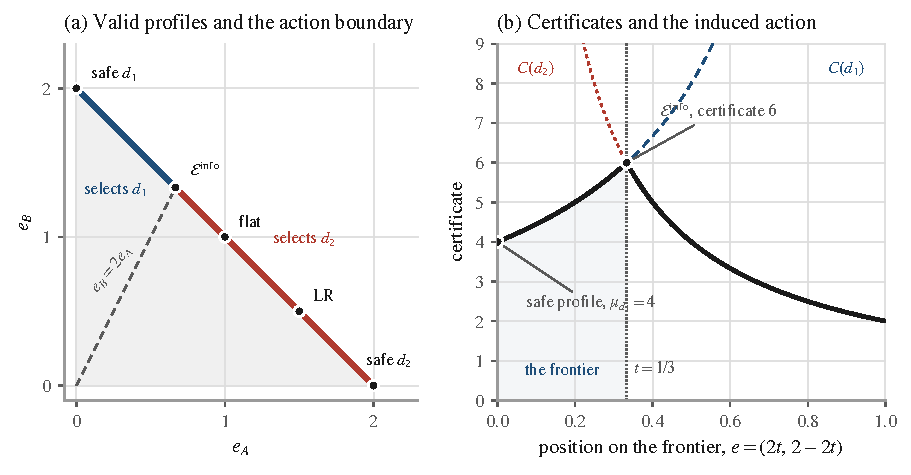
\includegraphics[width=0.92\textwidth]{toy_geometry.pdf}
\caption{Geometry of the two-outcome problem. Panel (a) shows the valid profiles and the action boundary, and panel (b) the two certificates along the budget line.}\label{fig:toy_geometry}
\end{figure}

Plotting the guarantee against the information gives the frontier in
Figure~\ref{fig:sim_frontier}. It is curved, so the exchange rate between the
two is not constant: the first units of certificate given up buy a great deal
of information, and the last buy very little. Most of the available
information can therefore be had for a modest loss of protection. The
protective endpoint itself is a limit of the curve rather than a point on it,
since the safe profile puts no e-value on $A$ and its log score is $-\infty$.

\begin{figure}[H]
\centering
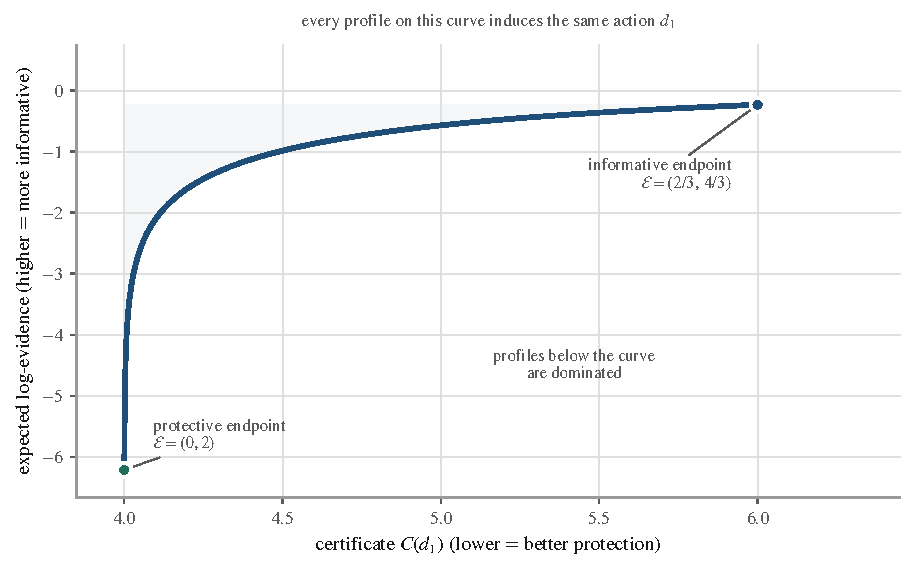
\includegraphics[width=0.92\textwidth]{sim_frontier.pdf}
\caption{The protection--information frontier for profiles inducing the bet on $A$.}\label{fig:sim_frontier}
\end{figure}

The same picture shows both cases of Proposition~\ref{prop:boundary}. Were
the target the hedge $d_2$, the likelihood ratio $(1.5,0.5)$, which sits at
$t=3/4$, would already lead to it, so the most informative profile for $d_2$
would be the ratio itself, with $d_2$ winning strictly at certificate $8/3$.
For the bet $d_1$ the ratio is out of reach, so the most informative profile
stops at the tie $t=1/3$. Which case applies depends only on whether the
likelihood ratio already leads to the target.

Where on the frontier to sit is a matter of preference, which the loss table
alone does not settle.

\subsection{Result 3: When Shape Functions Suffice}\label{sec:result3}

The first two results build profiles directly from the loss. The standard
construction never looks at the loss. It takes the likelihood ratio $r$ and
passes it through a shape function $w$, reporting $\mathcal E(z)=w(r(z))$.
Could a well-chosen shape function have produced the safe profile anyway? If
so, the loss would matter only for choosing $w$, and existing theory would
already cover the design problem.

There is a simple reason to doubt it. A shape function sees each outcome only
through its likelihood ratio, so two outcomes with the same ratio receive the
same score, however differently they cost. The safe profile scores outcomes
by their cost, so whenever two outcomes share a ratio but not a loss, no shape
function can reproduce it.

The shape functions used in practice come from the capped power family of
\citet{KoningvanMeer2025},
\begin{equation}
 w_h(r)=\min\!\left(\frac{r^{1/(1-h)}}{\lambda},\ \frac1\alpha\right).
 \label{eq:power_shape}
\end{equation}
It raises the ratio to a power, rescales it by the constant $\lambda$ that
makes the profile valid, and caps every score at $1/\alpha$. The parameter
$h<1$ sets how aggressively evidence is accumulated: $h=0$ returns the ratio
itself, and lower values flatten the profile. Different statisticians prefer
different $h$ and $\alpha$, but every member of the family reads each outcome
only through its ratio. The next result says exactly when that is enough.

\begin{proposition}[When shape functions suffice]\label{prop:no_shape}
Assume $\mu_d>0$, and let $r(z):=\widehat P_1(z)/P(z)$ be the likelihood ratio
against any fixed $P\in\mathcal P$ giving every outcome positive probability.
The safe profile $\mathcal E_d^{\mathrm{safe}}$ of
Theorem~\ref{thm:cert} can be written as $\mathcal E_d^{\mathrm{safe}}=w(r)$
for some function $w$ exactly when the loss is determined by the likelihood
ratio, meaning that
\[
  r(z)=r(z')\quad\text{implies}\quad L(d,z)=L(d,z')
\]
for every pair of outcomes $z,z'$.
\end{proposition}

\begin{proof}
Suppose first that $\mathcal E_d^{\mathrm{safe}}=w(r)$ for some $w$. If
$r(z)=r(z')$ then $w(r(z))=w(r(z'))$, so the two outcomes receive the same
e-value. Multiplying by $\mu_d$ recovers the loss, since
$L(d,\cdot)=\mu_d\,\mathcal E_d^{\mathrm{safe}}$, hence $L(d,z)=L(d,z')$.

Conversely, suppose the loss is constant on each level set of $r$. Define $w$
on the values $r$ actually takes by picking, for each such value $v$, any
outcome $z$ with $r(z)=v$ and setting
\[
  w(v)=\frac{L(d,z)}{\mu_d}.
\]
The choice of $z$ does not matter: any other outcome with the same ratio
carries the same loss by assumption, so $w$ is well defined. Off the range of
$r$ it may be given any values at all. By construction, at every outcome,
\[
  w(r(z))=\frac{L(d,z)}{\mu_d}=\mathcal E_d^{\mathrm{safe}}(z).
\]
\end{proof}

In words, a shape function can reproduce the safe profile exactly when
outcomes with the same likelihood ratio always carry the same loss. This can
fail in two different ways, and they should be kept apart.

The first is a failure of information. When two outcomes share a ratio but
differ in loss, nothing computed from the ratio can tell them apart, so no
shape function reproduces the safe profile, however it is chosen.

The second is subtler. When every outcome has its own ratio, the proposition
allows a suitable shape function to exist, but that function is only the loss
rewritten as a function of $r$ after the fact. A statistician choosing $w$
from preferences about evidence has no reason to arrive at it. Moreover, the
shape functions used in practice are increasing in $r$, so they give their
largest scores to the outcomes the belief rates likeliest relative to the
model, while the safe profile gives its largest scores to the outcomes where
the target is most expensive. When these are different outcomes, no
increasing shape can follow the safe profile, and
Section~\ref{sec:mkt_shape} shows a case where this alone puts the target out
of reach.

\subsection{The Procedure, Worked Through}\label{sec:recipe}

The three results combine into a procedure with three steps. First, compare
the actions and name the target. Second, build the safe profile for the
target. Third, if information matters, trade some protection for it while
keeping the target as a constraint. Each step is carried out below on the
two-outcome example, so every number can be checked by hand.

Step one compares the actions in the two ways a decision-maker might care
about, by worst-case expected loss across the model and by expected loss under
the belief. In the example,
\[
  \max_{P\in\mathcal P}\mathbb E_{P}[L(\cdot,Z)]
     =\bigl(\tfrac{0+8}{2},\tfrac{4+0}{2}\bigr)=(4,2),
  \qquad
  \mathbb E_{\widehat P_1}[L(\cdot,Z)]=(2,3),
\]
so the protective action is the hedge $d_2$, while the belief recommends the
bet $d_1$. The two differ, so the decision-maker has to choose. Take the bet
$d_1$ as the target, the choice of a belief-trusting decision-maker.
Everything that follows is conditional on that choice.

Step two builds the safe profile $L(d^\star,\cdot)/\mu_{d^\star}$. By
Theorem~\ref{thm:cert} it gives the target the strongest guarantee, and by
Corollary~\ref{cor:select} it leads to the target. For $d_1$, $\mu_{d_1}=4$
and $\mathcal E^{\mathrm{safe}}_{d_1}=(0,8)/4=(0,2)$, giving
\[
  C(d_1)=\max\bigl(0/0,\;8/2\bigr)=4,
  \qquad
  C(d_2)=\max\bigl(4/0,\;0/2\bigr)=\infty,
\]
under the conventions $0/0=0$ and $x/0=\infty$. The bet is selected. The
infinite certificate of the hedge is not an artefact. The safe profile puts
no e-value on $A$, the only outcome in which hedging costs anything, so that
loss is divided by zero rather than reduced.

Step three is optional. If the decision-maker also wants information, the
statistician moves along the frontier of Section~\ref{sec:frontier}, keeping
the target as a constraint. The most informative end is
$\mathcal E^{\mathrm{info}}=(2/3,4/3)$, with certificate $6$ instead of $4$ and
log score $-0.232$ instead of $-\infty$.

Table~\ref{tab:two_toy} collects the profiles. The two an evidence-first
statistician would report, the likelihood ratio and the flat profile, both
lead to the hedge. Only the profiles built from the loss of $d_1$ lead to the
bet. Each safe profile achieves its own action's best certificate and sends
the other action's to infinity, for the reason just seen.

\begin{table}[H]
\centering
\caption{Two-outcome profiles. $C_j$ is the certificate of action $d_j$.}\label{tab:two_toy}
\begin{tabular}{@{}l r r r r c@{}}\toprule
Profile & $\mathcal E(A)$ & $\mathcal E(B)$ & $C_1$ & $C_2$ & Action \\\midrule
Likelihood ratio & 1.50 & 0.50 & 16.00 & 2.67 & $d_2$ \\
Flat & 1.00 & 1.00 & 8.00 & 4.00 & $d_2$ \\
Safe for $d_2$ & 2.00 & 0.00 & $\infty$ & 2.00 & $d_2$ \\
Safe for $d_1$ & 0.00 & 2.00 & 4.00 & $\infty$ & $d_1$ \\
Informative for $d_1$ & 0.67 & 1.33 & 6.00 & 6.00 & $d_1$ \\\bottomrule
\end{tabular}
\end{table}

The last row is the informative profile. Its two certificates are equal, so
$d_1$ wins only through a tie, as Proposition~\ref{prop:boundary} predicts
when the likelihood ratio leads elsewhere. The three-outcome example behaves
the same way. Targeting $d_A$ there, the most informative profile is exactly
\[
  \mathcal E=\bigl(\tfrac95,\,\tfrac{12}{35},\,\tfrac67\bigr)
  \approx(1.80,\;0.34,\;0.86),
\]
with log score $+0.016$, and all three certificates equal
$35/3\approx11.67$, so $d_A$ ties with both competitors. A hand-picked profile that leans towards the draw,
$(0.3,0.7,2.0)$, also leads to $d_A$, and strictly, but scores $-0.760$.
Solving the constrained problem is therefore worth about $0.78$ in
log-evidence.

Every step of the procedure reads the loss. The likelihood ratio is still
worth reporting as a measure of evidence, but it is not a default the decision
should inherit.
